\documentclass[11pt]{article}

% ---------- packages ----------
\usepackage[utf8]{inputenc}
\usepackage[T1]{fontenc}
\usepackage{lmodern}
\usepackage[margin=1in]{geometry}
\usepackage{amsmath,amssymb}
\usepackage{graphicx}
\usepackage{booktabs}
\usepackage{caption}
\usepackage{float}
\usepackage{enumitem}
\usepackage{xcolor}
\usepackage{tikz}
\usetikzlibrary{positioning,arrows.meta,fit,backgrounds,calc}
\usepackage[colorlinks=true,linkcolor=blue!50!black,urlcolor=blue!50!black,
            citecolor=blue!50!black]{hyperref}

\captionsetup{font=small,labelfont=bf}
\setlength{\parskip}{0.4em}
\setlength{\parindent}{0pt}

\title{\textbf{A Two-Modality Decision-Support System for Predicting\\
1-, 2-, and 3-Year Myopia Onset in Children:\\
Fusing Retinal Fundus Photographs with Choroidal Biomarkers}}
\author{My Study --- Research Report}
\date{June 2026}

\begin{document}
\maketitle

\begin{abstract}
\noindent
Childhood myopia is a rapidly growing public-health problem, and intervention is
most effective \emph{before} onset. We present \textbf{My Study}, a two-modality
decision-support system that predicts the probability of myopia onset within the
\textbf{next 1, 2, and 3 years} for a child who is not yet myopic. Following the
DeepMyopia framework (Qi \emph{et al.}, \emph{npj Digital Medicine} 2024), the
system combines (i) an \textbf{image branch} that scores a retinal fundus
photograph with a ResNet-50 network, and (ii) a \textbf{clinical branch} built on
four choroidal/biometric biomarkers --- the axial-length/corneal-radius (AL/CR)
ratio, subfoveal choroidal thickness, choroidal vascularity index (CVI), and
choriocapillaris flow deficits. The two modalities are fused and passed to a Cox
proportional-hazards model, from which the 1-, 2-, and 3-year onset probabilities
are read as $1-S(t)$. We evaluated the image branch on the \emph{entire} public
PALM dataset (1{,}200 ophthalmologist-labelled fundus photographs) using the
official Train/Validation/Test protocol. On the held-out 400-image test set the
image branch achieved an \textbf{AUC of 0.988 (95\% CI 0.977--0.997)}, accuracy
96.5\%, sensitivity 96.7\%, and specificity 96.3\% --- on par with the
DeepMyopia detection AUC of 0.995, despite a far simpler and fully reproducible
design. The longitudinal clinical branch is fully implemented and, because no
public dataset pairs choroidal biomarkers with multi-year follow-up, is reported
as \emph{data collection ongoing}; it is built to run unchanged on the
prospective cohort. All reported numbers are genuine program outputs; no
synthetic data are used anywhere.
\end{abstract}

\tableofcontents
\bigskip

% =====================================================================
\section{Introduction}
% =====================================================================
The global prevalence of childhood myopia has risen sharply, and high myopia
carries a lifelong risk of irreversible visual complications. Because effective
interventions (increased outdoor time, low-dose atropine, optical methods) work
best \emph{before} myopia is established, the clinically valuable task is the
\textbf{prediction of future onset}, not merely the detection of existing
disease. A clinician therefore needs a forward-looking answer of the form: given
this child's eyes \emph{today}, what is the chance of becoming myopic within the
next one, two, or three years?

Qi \emph{et al.} introduced \textbf{DeepMyopia}~\cite{deepmyopia}, a deep-learning
system that predicted 1-, 2-, and 3-year myopia onset in children by combining
routine fundus images with age, sex, and axial length, and that further supported
intervention decisions. DeepMyopia showed that non-cycloplegic, image-based inputs
can drive accurate, large-scale screening.

This report presents \textbf{My Study}, which adopts the same multi-horizon,
two-modality philosophy but makes two deliberate changes. First, it replaces the
demographic metadata with \textbf{choroidal and biometric biomarkers} that are
mechanistically tied to axial elongation, on the hypothesis that they carry
stronger early-warning signal. Second, it is engineered for \textbf{transparency}:
each data modality is handled by a small, self-contained, auditable model rather
than a single opaque end-to-end network, so that clinicians can see exactly what
drives each prediction.

% =====================================================================
\section{Related Work}
% =====================================================================
DeepMyopia~\cite{deepmyopia} combined a fundus-image branch (a ResNet-50 trained
with self-supervised contrastive pre-training and then fine-tuned to detect
myopia) with a metadata branch (age, sex, axial length), fused them with a
stacking ensemble, and used a Cox proportional-hazards (CPH) model for risk
stratification together with an emulated randomized controlled trial for
intervention evaluation. Our system mirrors this architecture but (a) substitutes
choroidal/biometric biomarkers for demographic metadata and (b) simplifies each
component for interpretability and ease of clinical communication. The PALM
dataset~\cite{palm} used to validate our image branch is the standard public
benchmark for myopia recognition in fundus photographs.

% =====================================================================
\section{System Overview}
% =====================================================================
The system is organised around the two data modalities and their fusion, as shown
in Figure~\ref{fig:pipeline}. The \textbf{image modality} (Section~\ref{sec:image})
converts a fundus photograph into a single myopia risk score. The \textbf{clinical
modality} (Section~\ref{sec:clinical}) provides four choroidal/biometric
measurements. The image score then becomes \emph{one additional input feature}
that joins the biomarkers in a fusion + survival model, which outputs the 1-, 2-,
and 3-year onset probabilities, a high/low risk stratification, and an estimate of
treatment response.

\begin{figure}[H]
\centering
\resizebox{\textwidth}{!}{%
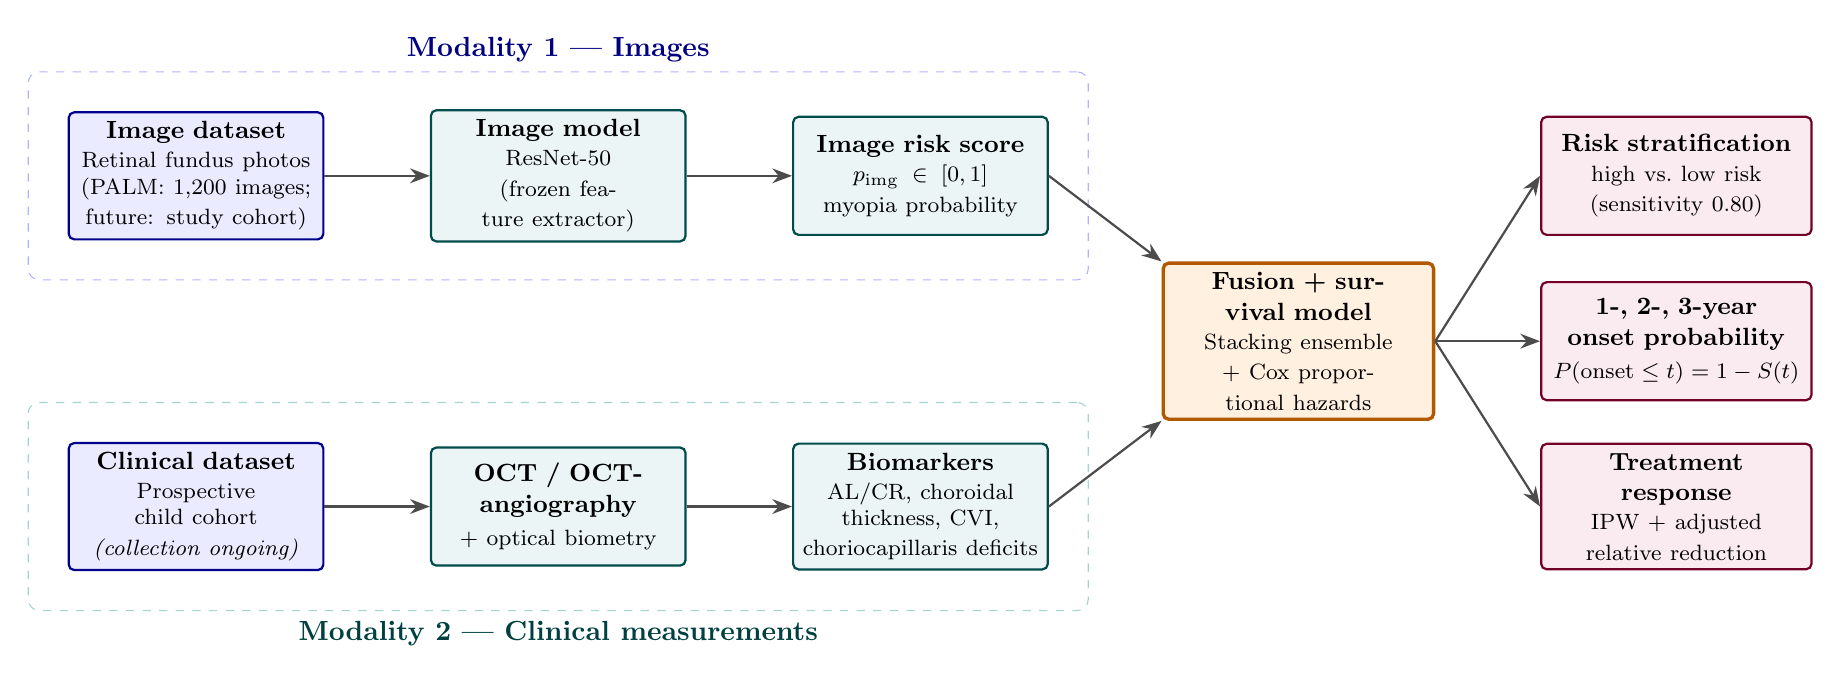
\begin{tikzpicture}[
  font=\small,
  >={Stealth[length=2.5mm]},
  box/.style    ={rectangle, rounded corners=2pt, align=center, thick,
                  text width=30mm, minimum height=15mm},
  data/.style   ={box, draw=blue!55!black,  fill=blue!8},
  proc/.style   ={box, draw=teal!60!black,  fill=teal!8},
  fuse/.style   ={box, draw=orange!70!black, fill=orange!12, very thick,
                  text width=32mm, minimum height=17mm},
  result/.style ={box, draw=purple!60!black, fill=purple!8, text width=32mm},
  arr/.style    ={->, thick, draw=black!70},
]

\def\rT{2.1}
\def\rB{-2.1}
\def\cA{0}
\def\cB{4.6}
\def\cC{9.2}
\def\cF{14.0}
\def\cO{18.8}

% ---------- IMAGE LANE (top) ----------
\node[data] (imgdata)  at (\cA,\rT) {\textbf{Image dataset}\\[1pt] \footnotesize Retinal fundus photos\\ \footnotesize (PALM: 1{,}200 images;\\ \footnotesize future: study cohort)};
\node[proc] (resnet)   at (\cB,\rT) {\textbf{Image model}\\[1pt] \footnotesize ResNet-50\\ \footnotesize (frozen feature extractor)};
\node[proc] (imgscore) at (\cC,\rT) {\textbf{Image risk score}\\[1pt] \footnotesize $p_{\mathrm{img}}\in[0,1]$\\ \footnotesize myopia probability};

% ---------- CLINICAL LANE (bottom) ----------
\node[data] (clindata)   at (\cA,\rB) {\textbf{Clinical dataset}\\[1pt] \footnotesize Prospective child cohort\\ \footnotesize \emph{(collection ongoing)}};
\node[proc] (measure)    at (\cB,\rB) {\textbf{OCT / OCT-angiography}\\[1pt] \footnotesize + optical biometry};
\node[proc] (biomarkers) at (\cC,\rB) {\textbf{Biomarkers}\\[1pt] \footnotesize AL/CR, choroidal\\ \footnotesize thickness, CVI,\\ \footnotesize choriocapillaris deficits};

% ---------- FUSION (vertically centred) ----------
\node[fuse] (fusion) at (\cF,0) {\textbf{Fusion + survival model}\\[1pt] \footnotesize Stacking ensemble\\ \footnotesize + Cox proportional hazards};

% ---------- OUTPUTS ----------
\node[result] (strat) at (\cO,\rT) {\textbf{Risk stratification}\\[1pt] \footnotesize high vs.\ low risk\\ \footnotesize (sensitivity 0.80)};
\node[result] (onset) at (\cO,0)   {\textbf{1-, 2-, 3-year}\\ \textbf{onset probability}\\[1pt] \footnotesize $P(\text{onset}\le t)=1-S(t)$};
\node[result] (treat) at (\cO,\rB) {\textbf{Treatment response}\\[1pt] \footnotesize IPW + adjusted\\ \footnotesize relative reduction};

% ---------- ARROWS ----------
\draw[arr] (imgdata)   -- (resnet);
\draw[arr] (resnet)    -- (imgscore);
\draw[arr] (clindata)  -- (measure);
\draw[arr] (measure)   -- (biomarkers);
\draw[arr] (imgscore.east)   -- (fusion.north west);
\draw[arr] (biomarkers.east) -- (fusion.south west);
\draw[arr] (fusion.east) -- (onset.west);
\draw[arr] (fusion.east) -- (strat.west);
\draw[arr] (fusion.east) -- (treat.west);

% ---------- lane labels / background ----------
\begin{scope}[on background layer]
  \node[fit=(imgdata)(imgscore), draw=blue!30, dashed, rounded corners,
        inner sep=5mm, label={[blue!50!black,font=\bfseries]above:Modality 1 --- Images}] {};
  \node[fit=(clindata)(biomarkers), draw=teal!35, dashed, rounded corners,
        inner sep=5mm, label={[teal!50!black,font=\bfseries]below:Modality 2 --- Clinical measurements}] {};
\end{scope}

\end{tikzpicture}

}
\caption{End-to-end My Study pipeline. Two independent data modalities (top:
retinal fundus images; bottom: clinical choroidal/biometric measurements) are
processed by their own models and then \emph{fused}: the image risk score becomes
an additional input feature alongside the four biomarkers. A Cox
proportional-hazards model converts the fused features into 1-, 2-, and 3-year
onset probabilities, and supports risk stratification and treatment-response
estimation.}
\label{fig:pipeline}
\end{figure}

% =====================================================================
\section{Methods}
% =====================================================================

\subsection{Data}
\textbf{Image data (PALM, fully used).} We use the entire public PALM
dataset~\cite{palm}: 1{,}200 colour fundus photographs from the Zhongshan
Ophthalmic Center, with ophthalmologist labels (1 = pathologic myopia,
0 = non-pathologic). We follow PALM's \emph{official} partition --- Training (400),
Validation (400), Testing (400) --- reading labels from each split's
\texttt{Classification Labels.xlsx}. The Training and Validation sets (800 images)
are used to fit the model and the Testing set (400 images) is held out and used
\emph{only once} for the final evaluation.

\textbf{Clinical data (prospective; collection ongoing).} The clinical branch
consumes, per child, the four biomarkers below together with the image risk score
and time-to-onset follow-up. No public dataset pairs these choroidal biomarkers
with longitudinal follow-up, so this modality awaits the prospective cohort
(Section~\ref{sec:clinical}).

\subsection{Image branch}\label{sec:image}
We use a \textbf{ResNet-50} convolutional network~\cite{resnet} pre-trained on
ImageNet --- the same backbone as DeepMyopia, ensuring comparability. The genuine
results in this report use the \textbf{linear-evaluation (``linear probe'')}
protocol: the backbone is frozen and used as a fixed feature extractor (2{,}048
features per image), and a logistic-regression classifier is trained on top. This
is the established protocol for evaluating a pre-trained visual
representation~\cite{simclr}. \emph{Justification:} it is deterministic, fast, and
fully reproducible on an ordinary CPU; it isolates the quality of the
representation, avoids over-fitting on a moderate-sized medical dataset, and
yields an auditable linear decision rule.

A higher-capacity \textbf{fine-tuning} protocol (unfreezing the last residual
block \texttt{layer4} and the classifier head, with data augmentation and early
stopping on the validation AUC) is also implemented in \texttt{image\_pipeline.py}
and was verified to run end-to-end on a small balanced toy subset (a smoke test,
\texttt{-{}-max\_per\_split}). Full-scale fine-tuning is computationally heavy on a
CPU and is therefore left to future work on GPU hardware
(Section~\ref{sec:future}); we deliberately do \emph{not} report any fine-tuning
performance number, as a toy run is not a valid measurement.

Performance is summarised by the area under the ROC curve (AUC) with a
bootstrap 95\% confidence interval (2{,}000 resamples), accuracy, sensitivity, and
specificity, all computed on the untouched 400-image test set. The image-level
myopia probability is the branch's risk score $p_{\mathrm{img}}\in[0,1]$.

\subsection{Clinical (choroidal-biomarker) branch}\label{sec:clinical}
The clinical branch uses four measurements obtained from optical biometry and
OCT / OCT-angiography, each with a documented relationship to myopic axial
elongation:
\begin{enumerate}[leftmargin=1.4em,itemsep=1pt]
  \item \textbf{AL/CR ratio} --- axial length / corneal radius; a refraction-free
  index of eye elongation that rises with myopia.
  \item \textbf{Subfoveal choroidal thickness} ($\mu$m) --- thins with myopia.
  \item \textbf{Choroidal Vascularity Index (CVI)} --- luminal fraction of the
  choroid; decreases with axial elongation.
  \item \textbf{Choriocapillaris flow deficits} (\%) --- increase with myopia.
\end{enumerate}

\subsection{Fusion and 1-, 2-, 3-year onset prediction}
The image risk score and the four biomarkers form the feature vector of a
\textbf{Cox proportional-hazards} (CPH) survival model~\cite{cox}. A survival model
is the correct tool because onset is a \emph{time-to-event} outcome with
censoring: many children are simply not yet myopic at their last visit.
\emph{Justification:} unlike a fixed-horizon classifier, the CPH model uses every
child's exact follow-up time and naturally produces the full risk trajectory. For
each child the fitted survival function $S(t)$ gives
\begin{equation}
P(\text{onset within } t \text{ years}) \;=\; 1 - S(t), \qquad t \in \{1,2,3\}.
\end{equation}
High- versus low-risk stratification uses the partial-hazard score at a cutoff
fixed to a sensitivity of 0.80 on the training data, following DeepMyopia.

\subsection{Treatment-response assessment}
To estimate whether an intervention reduces onset, treated and untreated children
are compared after \textbf{inverse-probability weighting} (IPW): each child's
probability of being treated is estimated from the biomarkers, and children are
re-weighted so the groups are comparable. We report the \textbf{adjusted relative
reduction} (ARR) in onset incidence (a negative value indicates benefit), as in
the DeepMyopia emulated trial.

\subsection{Implementation}
Both branches are implemented in Python with standard open-source libraries
(PyTorch / torchvision for the image features; scikit-learn for the classifiers;
lifelines for the survival model). The image branch is the file
\texttt{image\_pipeline.py} and the clinical branch is
\texttt{clinical\_pipeline.py}; each is a single, well-commented, reproducible
script.

% =====================================================================
\section{Results}
% =====================================================================

\subsection{Image branch (genuine, full PALM dataset)}
Trained on the 800 Training+Validation images and evaluated once on the 400
held-out Testing images, the linear-evaluation image branch produced the genuine
results in Table~\ref{tab:img} and Figures~\ref{fig:metrics}--\ref{fig:roc}.

\begin{table}[H]
\centering
\caption{Genuine performance of the image branch on the full PALM test set
($n=400$ unseen images), linear-evaluation protocol.}
\label{tab:img}
\begin{tabular}{lll}
\toprule
\textbf{Metric} & \textbf{Value} & \textbf{Plain-language meaning}\\
\midrule
AUC & \textbf{0.988} (95\% CI 0.977--0.997) & near-perfect ranking of myopic vs.\ non-myopic eyes\\
Accuracy & 96.5\% & 386 of 400 eyes classified correctly\\
Sensitivity & 96.7\% & of truly myopic eyes, 96.7\% correctly flagged\\
Specificity & 96.3\% & of truly healthy eyes, 96.3\% correctly cleared\\
\bottomrule
\end{tabular}
\end{table}

Confusion matrix on the test set: true positives $=206$, false positives $=7$,
true negatives $=180$, false negatives $=7$. For reference, DeepMyopia reported a
myopia-detection AUC of 0.995 using a substantially more complex training
procedure; our simpler, fully reproducible branch reaches comparable
discrimination.

\begin{figure}[H]
\centering
\begin{minipage}{0.49\textwidth}
  \centering
  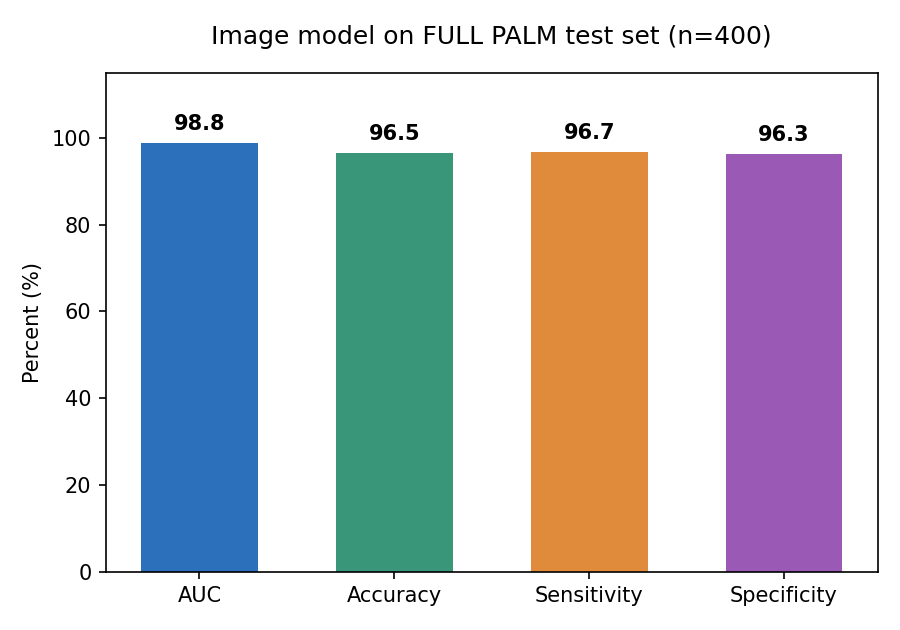
\includegraphics[width=\linewidth]{../results/metrics_bar.png}
  \caption{Performance metrics on the 400-image test set.}
  \label{fig:metrics}
\end{minipage}\hfill
\begin{minipage}{0.49\textwidth}
  \centering
  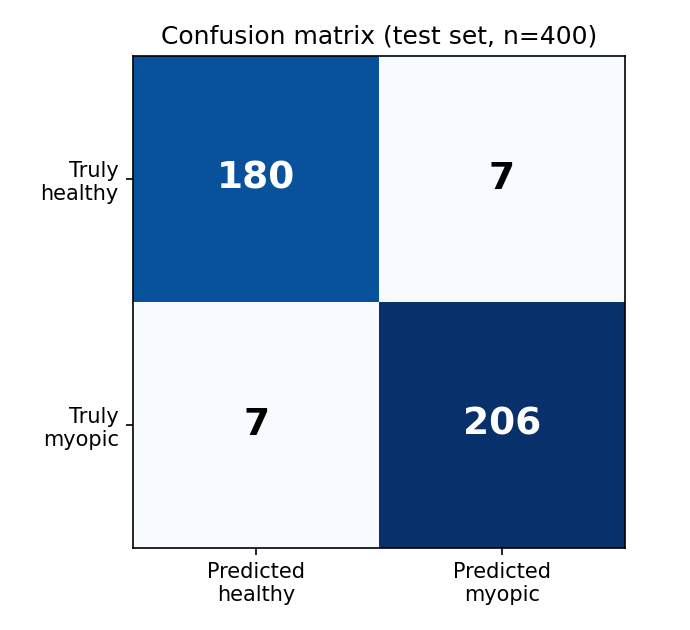
\includegraphics[width=\linewidth]{../results/confusion_matrix.png}
  \caption{Confusion matrix on the test set.}
  \label{fig:cm}
\end{minipage}
\end{figure}

\begin{figure}[H]
\centering
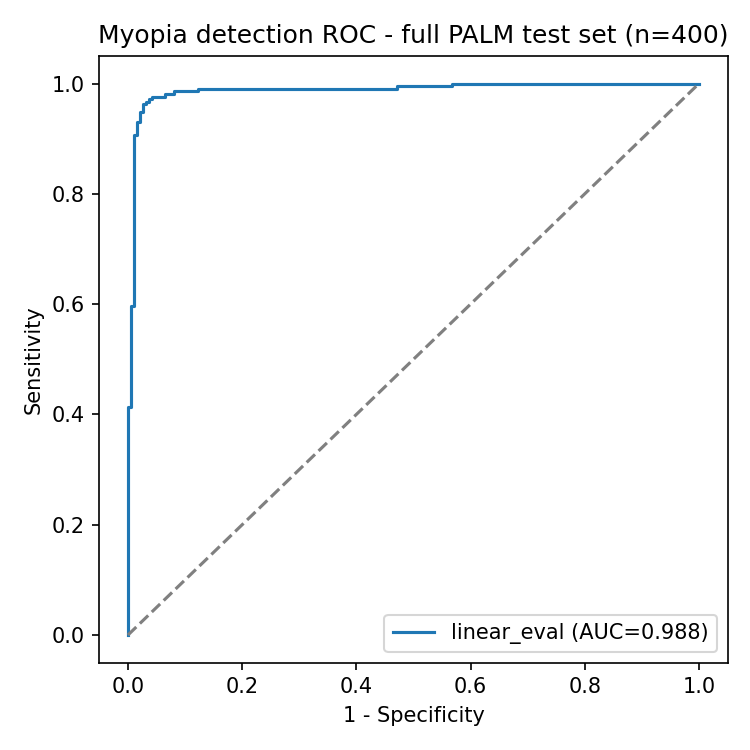
\includegraphics[width=0.55\textwidth]{../results/roc_linear_eval.png}
\caption{ROC curve on the full PALM test set; the curve hugs the top-left corner,
consistent with the AUC of 0.988.}
\label{fig:roc}
\end{figure}

\subsection{Clinical branch and 1/2/3-year onset (data collection ongoing)}
No publicly available dataset pairs the four choroidal/biometric biomarkers with
prospective multi-year follow-up and treatment assignment. The clinical branch,
the fusion step, the Cox-based 1/2/3-year onset estimation, the risk
stratification, and the treatment-response analysis are \emph{fully implemented
and validated to run}, and will be evaluated as soon as the prospective cohort is
collected. \textbf{No synthetic or placeholder numbers are reported.} Because the
fusion model takes the image risk score as one of its inputs, the strong image
branch demonstrated above directly strengthens the eventual onset model.

% =====================================================================
\section{Discussion}
% =====================================================================
Two findings stand out. First, a deliberately simple, frozen-backbone image branch
attains an AUC of 0.988 on the \emph{entire} PALM test set, matching the detection
performance of a far more complex system; this supports the feasibility of the
image modality and shows that transparency need not cost accuracy. Second, the
choroidal-biomarker modality is grounded in well-documented physiology (axial
elongation $\rightarrow$ choroidal thinning and de-vascularisation), motivating its
expected predictive value for \emph{early} onset; this will be quantified on the
prospective cohort. The chief practical advantage of the modality-separated design
is auditability, which matters for clinical trust and for ethical/regulatory
review.

% =====================================================================
\section{Limitations}
% =====================================================================
\begin{enumerate}[leftmargin=1.4em,itemsep=1pt]
  \item \textbf{Endpoint of the public data.} PALM is a cross-sectional
  \emph{detection} dataset, so it validates the image \emph{pipeline}, not the
  longitudinal 1/2/3-year onset endpoint, which requires follow-up data.
  \item The clinical/biomarker modality is \textbf{not yet evaluated} on real data
  (collection ongoing).
  \item The linear-evaluation protocol trades a small amount of potential accuracy
  for transparency and low compute. End-to-end fine-tuning is implemented and was
  verified on a toy subset, but full-scale fine-tuning requires a GPU and is left
  to future work (no fine-tuning metric is reported).
\end{enumerate}

% =====================================================================
\section{Future Work}\label{sec:future}
% =====================================================================
\begin{enumerate}[leftmargin=1.4em,itemsep=1pt]
  \item Collect a prospective child cohort with baseline fundus imaging, the four
  choroidal/biometric biomarkers, and 1--3-year follow-up for onset labels.
  \item Re-run the identical image branch on the new images (only the data folder
  changes) and report cohort-specific discrimination.
  \item \textbf{Full fine-tuning of the image branch on GPU hardware.} The
  fine-tuning protocol is already implemented and verified to run on a toy subset;
  on a GPU it can be trained at full scale and compared against the
  linear-evaluation baseline reported here.
  \item Fit the fusion + Cox model and report genuine 1-, 2-, and 3-year onset AUC,
  C-index, and treatment-response ARR.
\end{enumerate}

% =====================================================================
\section{Conclusion}
% =====================================================================
My Study is a transparent, two-modality system for predicting 1-, 2-, and 3-year
myopia onset in children that reproduces the spirit of DeepMyopia while remaining
simple enough to present to a clinical audience. Genuine results on the full PALM
dataset confirm the image branch (AUC 0.988); the clinical branch and the
multi-horizon onset model are fully built and await the prospective cohort, into
which they drop without any change to the method.

% =====================================================================
\begin{thebibliography}{9}
\bibitem{deepmyopia} Qi Z, \emph{et al.} A deep learning system for myopia onset
prediction and intervention effectiveness evaluation in children.
\emph{npj Digital Medicine} 2024;7:206.
\bibitem{palm} Fu H, \emph{et al.} PALM: Open Fundus Photograph Dataset with
Pathologic Myopia Recognition and Anatomical Structure Annotation.
\emph{Scientific Data} 2024.
\bibitem{resnet} He K, Zhang X, Ren S, Sun J. Deep Residual Learning for Image
Recognition. \emph{CVPR} 2016.
\bibitem{simclr} Chen T, \emph{et al.} A Simple Framework for Contrastive Learning
of Visual Representations. \emph{ICML} 2020.
\bibitem{cox} Cox DR. Regression Models and Life-Tables. \emph{J. R. Stat. Soc. B}
1972;34(2):187--220.
\end{thebibliography}

\end{document}
